% Options for packages loaded elsewhere
\PassOptionsToPackage{unicode}{hyperref}
\PassOptionsToPackage{hyphens}{url}
%
\documentclass[
]{article}
\usepackage{lmodern}
\usepackage{amssymb,amsmath}
\usepackage{ifxetex,ifluatex}
\ifnum 0\ifxetex 1\fi\ifluatex 1\fi=0 % if pdftex
  \usepackage[T1]{fontenc}
  \usepackage[utf8]{inputenc}
  \usepackage{textcomp} % provide euro and other symbols
\else % if luatex or xetex
  \usepackage{unicode-math}
  \defaultfontfeatures{Scale=MatchLowercase}
  \defaultfontfeatures[\rmfamily]{Ligatures=TeX,Scale=1}
\fi
% Use upquote if available, for straight quotes in verbatim environments
\IfFileExists{upquote.sty}{\usepackage{upquote}}{}
\IfFileExists{microtype.sty}{% use microtype if available
  \usepackage[]{microtype}
  \UseMicrotypeSet[protrusion]{basicmath} % disable protrusion for tt fonts
}{}
\makeatletter
\@ifundefined{KOMAClassName}{% if non-KOMA class
  \IfFileExists{parskip.sty}{%
    \usepackage{parskip}
  }{% else
    \setlength{\parindent}{0pt}
    \setlength{\parskip}{6pt plus 2pt minus 1pt}}
}{% if KOMA class
  \KOMAoptions{parskip=half}}
\makeatother
\usepackage{xcolor}
\IfFileExists{xurl.sty}{\usepackage{xurl}}{} % add URL line breaks if available
\IfFileExists{bookmark.sty}{\usepackage{bookmark}}{\usepackage{hyperref}}
\hypersetup{
  pdftitle={Lesson 04 - Getting Started with R},
  hidelinks,
  pdfcreator={LaTeX via pandoc}}
\urlstyle{same} % disable monospaced font for URLs
\usepackage[margin=1in]{geometry}
\usepackage{color}
\usepackage{fancyvrb}
\newcommand{\VerbBar}{|}
\newcommand{\VERB}{\Verb[commandchars=\\\{\}]}
\DefineVerbatimEnvironment{Highlighting}{Verbatim}{commandchars=\\\{\}}
% Add ',fontsize=\small' for more characters per line
\usepackage{framed}
\definecolor{shadecolor}{RGB}{248,248,248}
\newenvironment{Shaded}{\begin{snugshade}}{\end{snugshade}}
\newcommand{\AlertTok}[1]{\textcolor[rgb]{0.94,0.16,0.16}{#1}}
\newcommand{\AnnotationTok}[1]{\textcolor[rgb]{0.56,0.35,0.01}{\textbf{\textit{#1}}}}
\newcommand{\AttributeTok}[1]{\textcolor[rgb]{0.77,0.63,0.00}{#1}}
\newcommand{\BaseNTok}[1]{\textcolor[rgb]{0.00,0.00,0.81}{#1}}
\newcommand{\BuiltInTok}[1]{#1}
\newcommand{\CharTok}[1]{\textcolor[rgb]{0.31,0.60,0.02}{#1}}
\newcommand{\CommentTok}[1]{\textcolor[rgb]{0.56,0.35,0.01}{\textit{#1}}}
\newcommand{\CommentVarTok}[1]{\textcolor[rgb]{0.56,0.35,0.01}{\textbf{\textit{#1}}}}
\newcommand{\ConstantTok}[1]{\textcolor[rgb]{0.00,0.00,0.00}{#1}}
\newcommand{\ControlFlowTok}[1]{\textcolor[rgb]{0.13,0.29,0.53}{\textbf{#1}}}
\newcommand{\DataTypeTok}[1]{\textcolor[rgb]{0.13,0.29,0.53}{#1}}
\newcommand{\DecValTok}[1]{\textcolor[rgb]{0.00,0.00,0.81}{#1}}
\newcommand{\DocumentationTok}[1]{\textcolor[rgb]{0.56,0.35,0.01}{\textbf{\textit{#1}}}}
\newcommand{\ErrorTok}[1]{\textcolor[rgb]{0.64,0.00,0.00}{\textbf{#1}}}
\newcommand{\ExtensionTok}[1]{#1}
\newcommand{\FloatTok}[1]{\textcolor[rgb]{0.00,0.00,0.81}{#1}}
\newcommand{\FunctionTok}[1]{\textcolor[rgb]{0.00,0.00,0.00}{#1}}
\newcommand{\ImportTok}[1]{#1}
\newcommand{\InformationTok}[1]{\textcolor[rgb]{0.56,0.35,0.01}{\textbf{\textit{#1}}}}
\newcommand{\KeywordTok}[1]{\textcolor[rgb]{0.13,0.29,0.53}{\textbf{#1}}}
\newcommand{\NormalTok}[1]{#1}
\newcommand{\OperatorTok}[1]{\textcolor[rgb]{0.81,0.36,0.00}{\textbf{#1}}}
\newcommand{\OtherTok}[1]{\textcolor[rgb]{0.56,0.35,0.01}{#1}}
\newcommand{\PreprocessorTok}[1]{\textcolor[rgb]{0.56,0.35,0.01}{\textit{#1}}}
\newcommand{\RegionMarkerTok}[1]{#1}
\newcommand{\SpecialCharTok}[1]{\textcolor[rgb]{0.00,0.00,0.00}{#1}}
\newcommand{\SpecialStringTok}[1]{\textcolor[rgb]{0.31,0.60,0.02}{#1}}
\newcommand{\StringTok}[1]{\textcolor[rgb]{0.31,0.60,0.02}{#1}}
\newcommand{\VariableTok}[1]{\textcolor[rgb]{0.00,0.00,0.00}{#1}}
\newcommand{\VerbatimStringTok}[1]{\textcolor[rgb]{0.31,0.60,0.02}{#1}}
\newcommand{\WarningTok}[1]{\textcolor[rgb]{0.56,0.35,0.01}{\textbf{\textit{#1}}}}
\usepackage{graphicx,grffile}
\makeatletter
\def\maxwidth{\ifdim\Gin@nat@width>\linewidth\linewidth\else\Gin@nat@width\fi}
\def\maxheight{\ifdim\Gin@nat@height>\textheight\textheight\else\Gin@nat@height\fi}
\makeatother
% Scale images if necessary, so that they will not overflow the page
% margins by default, and it is still possible to overwrite the defaults
% using explicit options in \includegraphics[width, height, ...]{}
\setkeys{Gin}{width=\maxwidth,height=\maxheight,keepaspectratio}
% Set default figure placement to htbp
\makeatletter
\def\fps@figure{htbp}
\makeatother
\setlength{\emergencystretch}{3em} % prevent overfull lines
\providecommand{\tightlist}{%
  \setlength{\itemsep}{0pt}\setlength{\parskip}{0pt}}
\setcounter{secnumdepth}{-\maxdimen} % remove section numbering

\title{Lesson 04 - Getting Started with R}
\author{}
\date{\vspace{-2.5em}\emph{Last Updated 08-14-2020}}

\begin{document}
\maketitle

\hypertarget{introduction}{%
\section{Introduction}\label{introduction}}

This lesson is designed to explain the basics of how R works as a
programming language.

\hypertarget{learning-objectives}{%
\subsubsection{Learning Objectives}\label{learning-objectives}}

\begin{itemize}
\tightlist
\item
  Define the following terms as they relate to R: object, assign, call,
  function, arguments, options.
\item
  Assign values to objects in R.
\item
  Learn how to \emph{name} objects
\item
  Solve simple arithmetic operations in R.
\item
  Call functions and use arguments to change their default options.
\item
  Inspect the content of vectors and manipulate their content.
\item
  Subset and extract values from vectors.
\item
  Write logical statements that resolve as TRUE and FALSE.
\item
  Describe what a data frame is.
\item
  Summarize the contents of a data frame.
\item
  Extract vectors out of data frames using variable names.
\end{itemize}

\begin{center}\rule{0.5\linewidth}{0.5pt}\end{center}

\hypertarget{writing-scripts}{%
\section{Writing Scripts}\label{writing-scripts}}

In lesson 02 we saw that we could write R code in the console and get
immediate results. There are two main ways of interacting with R: by
using the console or by using script files (plain text files that
contain your code). We will be working in R markdown files exclusively
in this class, but it is important to be aware that there are also
script files that have an extension of \texttt{.R}. These can contain
code and comments only, not normal text sentences like this.

Because we want our code and workflow to be reproducible, and often your
code may span several lines at a time, it is better to type the commands
we want in a script, and save the script. This way, there is a complete
record of what we did, and anyone (including our future selves!) can
easily replicate the results on their computer. It's also easier to fix
mistakes this way, without having to retype in the entire command.

\hypertarget{start-a-new-rmarkdown-file}{%
\subparagraph{Start a new Rmarkdown
file}\label{start-a-new-rmarkdown-file}}

\begin{itemize}
\tightlist
\item
  Go to File --\textgreater{} New File --\textgreater{} R Markdown to
  open a new R markdown window.
\item
  Give this file a name such as ``Lesson 04 notes'', and put your name
  as the author.
\item
  Delete all the template language below line 11.
\end{itemize}

Now let's go back to that long expression from lesson 2 (corrected), but
this time type it into a new code chunk. Recall we can make a new code
chunk by pressing \texttt{CTRL}+\texttt{ALT}+\texttt{I}, or by clicking
on \emph{Insert} then \emph{R}. Also recall that we submit this code by
pressing \texttt{Ctrl}+\texttt{Enter} or clicking the green play arrow
in the top right corner of the code chunk.

\begin{verbatim}
2 + 5*(8^3)- 3*log(10)
\end{verbatim}

\hypertarget{make-a-change-to-the-above-expression-and-run-the-command-again.}{%
\subparagraph{Make a change to the above expression and run the command
again.}\label{make-a-change-to-the-above-expression-and-run-the-command-again.}}

For the rest of this lesson, retype each code chunk below into the notes
file you just created. Be sure to annotate these notes as you would take
notes in any other class. For you to retain what you are reading and
learning, writing out what these pieces of code are doing (e.g.~the
assignment operator \texttt{\textless{}-}) in \textbf{your own words} is
an effective learning technique.

\begin{center}\rule{0.5\linewidth}{0.5pt}\end{center}

\hypertarget{creating-objects-in-r}{%
\section{Creating objects in R}\label{creating-objects-in-r}}

To do useful and interesting things, we need to assign \emph{values} to
\emph{objects}. To create an object, we need to give it a name followed
by the assignment operator \texttt{\textless{}-}, and the value we want
to give it:

\begin{Shaded}
\begin{Highlighting}[]
\NormalTok{weight_kg <-}\StringTok{ }\DecValTok{55}
\end{Highlighting}
\end{Shaded}

\texttt{\textless{}-} is the assignment operator. It assigns values on
the right to objects on the left. So, after executing
\texttt{x\ \textless{}-\ 3}, the value of \texttt{x} is \texttt{3}.

\textbf{Objects can be given any name such as \texttt{x},
\texttt{current\_temperature}, or \texttt{subject\_id}. However there
are some naming guidelines you need to be aware of.}

\begin{itemize}
\tightlist
\item
  You want your object names to be explicit and not too long.
\item
  They cannot start with a number (\texttt{2x} is not valid, but
  \texttt{x2} is).
\item
  R is case sensitive (e.g., \texttt{weight\_kg} is different from
  \texttt{Weight\_kg}).
\item
  There are some names that cannot be used because they are the names of
  fundamental functions in R (e.g., \texttt{if}, \texttt{else},
  \texttt{for}, see
  \href{https://stat.ethz.ch/R-manual/R-devel/library/base/html/Reserved.html}{here}
  for a complete list).
\item
  It's best to not use other function names (e.g., \texttt{c},
  \texttt{T}, \texttt{mean}, \texttt{data}, \texttt{df},
  \texttt{weights}) because these already tend to be in use by different
  parts of R.
\item
  See \href{https://google.github.io/styleguide/Rguide.xml}{Google's}
  style guide for more information.
\end{itemize}

When assigning a value to an object, R does not print anything. You can
force R to print the value by using parentheses or by typing the object
name:

\begin{Shaded}
\begin{Highlighting}[]
\NormalTok{weight_kg <-}\StringTok{ }\DecValTok{55}    \CommentTok{# doesn't print anything}
\NormalTok{(weight_kg <-}\StringTok{ }\DecValTok{55}\NormalTok{)  }\CommentTok{# but putting parenthesis around the call prints the value of `weight_kg`}
\end{Highlighting}
\end{Shaded}

\begin{verbatim}
## [1] 55
\end{verbatim}

\begin{Shaded}
\begin{Highlighting}[]
\NormalTok{weight_kg          }\CommentTok{# and so does typing the name of the object}
\end{Highlighting}
\end{Shaded}

\begin{verbatim}
## [1] 55
\end{verbatim}

Now that R has \texttt{weight\_kg} in memory, we can do arithmetic with
it. For instance, we may want to convert this weight into pounds (weight
in pounds is 2.2 times the weight in kg):

\begin{Shaded}
\begin{Highlighting}[]
\FloatTok{2.2} \OperatorTok{*}\StringTok{ }\NormalTok{weight_kg}
\end{Highlighting}
\end{Shaded}

\begin{verbatim}
## [1] 121
\end{verbatim}

We can also change an object's value by assigning it a new one:

\begin{Shaded}
\begin{Highlighting}[]
\NormalTok{weight_kg <-}\StringTok{ }\FloatTok{57.5}
\FloatTok{2.2} \OperatorTok{*}\StringTok{ }\NormalTok{weight_kg}
\end{Highlighting}
\end{Shaded}

\begin{verbatim}
## [1] 126.5
\end{verbatim}

This means that assigning a value to one object does not change the
values of other objects For example, let's store the animal's weight in
pounds in a new object, \texttt{weight\_lb}:

\begin{Shaded}
\begin{Highlighting}[]
\NormalTok{weight_lb <-}\StringTok{ }\FloatTok{2.2} \OperatorTok{*}\StringTok{ }\NormalTok{weight_kg}
\end{Highlighting}
\end{Shaded}

and then change \texttt{weight\_kg} to 100.

\begin{Shaded}
\begin{Highlighting}[]
\NormalTok{weight_kg <-}\StringTok{ }\DecValTok{100}
\end{Highlighting}
\end{Shaded}

R executes code in top-down order. So what happens on line 10 occurs
before line 11. What do you think is the current content of the object
\texttt{weight\_lb}? 126.5 or 220?

\emph{\textbf{Comments.}} \emph{The comment character in R is
\texttt{\#}, anything to the right of a \texttt{\#} in a script will be
ignored by R. It is useful to leave notes, and explanations in your
scripts as demonstrated earlier.}

\begin{center}\rule{0.5\linewidth}{0.5pt}\end{center}

\hypertarget{functions-and-their-arguments}{%
\section{Functions and their
arguments}\label{functions-and-their-arguments}}

Functions are ``canned scripts'' that automate more complicated sets of
commands including operations assignments, etc. Many functions are
predefined, or can be made available by importing R \emph{packages}
(lesson 02).

A function usually takes one or more inputs called \emph{arguments}, and
often (but not always) return a \emph{value}.

A typical example would be the function \texttt{sqrt()}. The input is
the number \texttt{4}, and the return value (the output) is the square
root of 4, namely 2. Executing a function (`running it') is called
\emph{calling} the function.

\begin{Shaded}
\begin{Highlighting}[]
\KeywordTok{sqrt}\NormalTok{(}\DecValTok{4}\NormalTok{)}
\end{Highlighting}
\end{Shaded}

\begin{verbatim}
## [1] 2
\end{verbatim}

Let's look into the \texttt{round} function.

\begin{Shaded}
\begin{Highlighting}[]
\KeywordTok{round}\NormalTok{(}\FloatTok{3.14159}\NormalTok{)}
\end{Highlighting}
\end{Shaded}

\begin{verbatim}
## [1] 3
\end{verbatim}

We can learn more about this function by typing \texttt{?round}. The
\textbf{Usage} section of the help documentation shows you what the
default values for each argument are. This is a very important piece to
pay attention. Sometimes the default behaviors are not what you want to
happen.

\begin{Shaded}
\begin{Highlighting}[]
\KeywordTok{round}\NormalTok{(x, }\DataTypeTok{digits=}\DecValTok{0}\NormalTok{)}
\end{Highlighting}
\end{Shaded}

In the \textbf{Arguments} section the help file defines what each
argument does.

\begin{itemize}
\tightlist
\item
  \texttt{x} is the object that you want to round. It must be a
  \emph{numeric vector}.
\item
  \texttt{digits} is an integer indicating the number of decimal places
  to round to.
\end{itemize}

Above, we called \texttt{round()} with just one argument,
\texttt{3.14159}, and it has returned the value \texttt{3}. That's
because the default is to round to the nearest whole number. We see that
if we want a different number of digits, we can type
\texttt{digits\ =\ 2} or however many we want.

\begin{Shaded}
\begin{Highlighting}[]
\KeywordTok{round}\NormalTok{(}\FloatTok{3.14159}\NormalTok{, }\DataTypeTok{digits =} \DecValTok{2}\NormalTok{)}
\end{Highlighting}
\end{Shaded}

\begin{verbatim}
## [1] 3.14
\end{verbatim}

If you provide the arguments in the exact same order as they are defined
you don't have to name them:

\begin{Shaded}
\begin{Highlighting}[]
\KeywordTok{round}\NormalTok{(}\FloatTok{3.14159}\NormalTok{, }\DecValTok{2}\NormalTok{)}
\end{Highlighting}
\end{Shaded}

\begin{verbatim}
## [1] 3.14
\end{verbatim}

And if you do name the arguments, you can switch their order:

\begin{Shaded}
\begin{Highlighting}[]
\KeywordTok{round}\NormalTok{(}\DataTypeTok{digits =} \DecValTok{2}\NormalTok{, }\DataTypeTok{x =} \FloatTok{3.14159}\NormalTok{)}
\end{Highlighting}
\end{Shaded}

\begin{verbatim}
## [1] 3.14
\end{verbatim}

This is a simple function with only one argument. Functions are the
backbone of how R does it's thing. You will get lots of practice with
functions, and quickly encounter functions that require many arguments.

\begin{center}\rule{0.5\linewidth}{0.5pt}\end{center}

\hypertarget{vectors-and-data-types}{%
\section{Vectors and data types}\label{vectors-and-data-types}}

A vector is the most common and basic data type in R, and is pretty much
the workhorse of R. A vector is composed by a series of values, which
can be either numbers or characters. We can assign a series of values to
a vector using the \texttt{c()} function. For example we can create a
vector of animal weights and assign it to a new object
\texttt{weight\_g}:

\begin{Shaded}
\begin{Highlighting}[]
\NormalTok{(weight_g <-}\StringTok{ }\KeywordTok{c}\NormalTok{(}\DecValTok{50}\NormalTok{, }\DecValTok{60}\NormalTok{, }\DecValTok{65}\NormalTok{, }\DecValTok{82}\NormalTok{))}
\end{Highlighting}
\end{Shaded}

\begin{verbatim}
## [1] 50 60 65 82
\end{verbatim}

A vector can also contain characters:

\begin{Shaded}
\begin{Highlighting}[]
\NormalTok{(animals <-}\StringTok{ }\KeywordTok{c}\NormalTok{(}\StringTok{"mouse"}\NormalTok{, }\StringTok{"rat"}\NormalTok{, }\StringTok{"dog"}\NormalTok{))}
\end{Highlighting}
\end{Shaded}

\begin{verbatim}
## [1] "mouse" "rat"   "dog"
\end{verbatim}

The quotes around ``mouse'', ``rat'', etc. are essential here. Without
the quotes R will assume objects have been created called
\texttt{mouse}, \texttt{rat} and \texttt{dog}. As these objects don't
exist in R's memory, there will be an error message.

An important feature of a vector, is that all of the elements are the
same type of data. The function \texttt{class()} indicates the class
(the type of element) of an object:

\begin{Shaded}
\begin{Highlighting}[]
\KeywordTok{class}\NormalTok{(weight_g)}
\end{Highlighting}
\end{Shaded}

\begin{verbatim}
## [1] "numeric"
\end{verbatim}

\begin{Shaded}
\begin{Highlighting}[]
\KeywordTok{class}\NormalTok{(animals)}
\end{Highlighting}
\end{Shaded}

\begin{verbatim}
## [1] "character"
\end{verbatim}

The function \texttt{str()} provides an overview of the structure of an
object and its elements. It is a useful function when working with large
and complex objects:

\begin{Shaded}
\begin{Highlighting}[]
\KeywordTok{str}\NormalTok{(weight_g)}
\end{Highlighting}
\end{Shaded}

\begin{verbatim}
##  num [1:4] 50 60 65 82
\end{verbatim}

\begin{Shaded}
\begin{Highlighting}[]
\KeywordTok{str}\NormalTok{(animals)}
\end{Highlighting}
\end{Shaded}

\begin{verbatim}
##  chr [1:3] "mouse" "rat" "dog"
\end{verbatim}

\hypertarget{data-types}{%
\subsection{Data Types}\label{data-types}}

R objects come in different data types. You just saw vectors comprised
of numbers (\textbf{numeric}), of words (\textbf{character} or
\textbf{string}). The other common data type that we will be
encountering in this class is a \texttt{"logical"} (sometimes called
Boolean). These are created by writing a logical statement where the
answer is either TRUE or FALSE. Silly examples include ``Is 3 greater
than 4?'' and ``Is the square root of 4 equal to 2?''

\begin{Shaded}
\begin{Highlighting}[]
\DecValTok{3}\OperatorTok{>}\DecValTok{4}
\end{Highlighting}
\end{Shaded}

\begin{verbatim}
## [1] FALSE
\end{verbatim}

\begin{Shaded}
\begin{Highlighting}[]
\KeywordTok{sqrt}\NormalTok{(}\DecValTok{4}\NormalTok{)}\OperatorTok{==}\DecValTok{2}
\end{Highlighting}
\end{Shaded}

\begin{verbatim}
## [1] TRUE
\end{verbatim}

We will see how to use these logical statements to do things such as
subsetting data and creating new variables.

Vectors are one of the many \textbf{data structures} that R uses. Other
important ones are lists (\texttt{list}), matrices (\texttt{matrix}),
data frames (\texttt{data.frame}), factors (\texttt{factor}) and arrays
(\texttt{array}). We will only talk about \texttt{data.frame}s and
\texttt{factors} in this class.

\hypertarget{doing-math-on-vectors}{%
\subsection{Doing math on vectors}\label{doing-math-on-vectors}}

You can perform math operations on the elements of a vector such as

\begin{Shaded}
\begin{Highlighting}[]
\NormalTok{weight_KG <-}\StringTok{ }\NormalTok{weight_g}\OperatorTok{/}\DecValTok{1000}
\NormalTok{weight_KG}
\end{Highlighting}
\end{Shaded}

\begin{verbatim}
## [1] 0.050 0.060 0.065 0.082
\end{verbatim}

When adding two vectors together, the elements in the same position are
added to each other. So element 1 in the vector \texttt{a} is added to
element 1 in vector \texttt{b}.

\begin{Shaded}
\begin{Highlighting}[]
\NormalTok{a <-}\StringTok{ }\KeywordTok{c}\NormalTok{(}\DecValTok{1}\NormalTok{,}\DecValTok{2}\NormalTok{,}\DecValTok{3}\NormalTok{)}
\NormalTok{b <-}\StringTok{ }\KeywordTok{c}\NormalTok{(}\DecValTok{6}\NormalTok{,}\DecValTok{7}\NormalTok{,}\DecValTok{8}\NormalTok{)}
\NormalTok{a}\OperatorTok{+}\NormalTok{b}
\end{Highlighting}
\end{Shaded}

\begin{verbatim}
## [1]  7  9 11
\end{verbatim}

More complex calculations can be performed on multiple vectors.

\begin{Shaded}
\begin{Highlighting}[]
\NormalTok{wt_lb <-}\StringTok{ }\KeywordTok{c}\NormalTok{(}\DecValTok{155}\NormalTok{, }\DecValTok{135}\NormalTok{, }\DecValTok{90}\NormalTok{)}
\NormalTok{ht_in <-}\StringTok{ }\KeywordTok{c}\NormalTok{(}\DecValTok{72}\NormalTok{, }\DecValTok{64}\NormalTok{, }\DecValTok{50}\NormalTok{)}
\NormalTok{bmi <-}\StringTok{ }\DecValTok{703}\OperatorTok{*}\NormalTok{wt_lb }\OperatorTok{/}\StringTok{ }\NormalTok{ht_in}\OperatorTok{^}\DecValTok{2}
\NormalTok{bmi}
\end{Highlighting}
\end{Shaded}

\begin{verbatim}
## [1] 21.01948 23.17017 25.30800
\end{verbatim}

All these operations on vectors behave the same way when dealing with
variables in a data set (data.frame).

If you want to add the values \emph{within} a vector, you use functions
such as \texttt{sum()}, \texttt{max()} and \texttt{mean()}

\begin{Shaded}
\begin{Highlighting}[]
\KeywordTok{sum}\NormalTok{(a)}
\end{Highlighting}
\end{Shaded}

\begin{verbatim}
## [1] 6
\end{verbatim}

\begin{Shaded}
\begin{Highlighting}[]
\KeywordTok{max}\NormalTok{(b)}
\end{Highlighting}
\end{Shaded}

\begin{verbatim}
## [1] 8
\end{verbatim}

\begin{Shaded}
\begin{Highlighting}[]
\KeywordTok{mean}\NormalTok{(a}\OperatorTok{+}\NormalTok{b)}
\end{Highlighting}
\end{Shaded}

\begin{verbatim}
## [1] 9
\end{verbatim}

\hypertarget{subsetting-vectors}{%
\subsection{Subsetting vectors}\label{subsetting-vectors}}

If we want to extract one or several values from a vector, we must
provide one or several indices in square brackets. For instance:

\begin{Shaded}
\begin{Highlighting}[]
\NormalTok{animals <-}\StringTok{ }\KeywordTok{c}\NormalTok{(}\StringTok{"mouse"}\NormalTok{, }\StringTok{"rat"}\NormalTok{, }\StringTok{"dog"}\NormalTok{, }\StringTok{"cat"}\NormalTok{)}
\NormalTok{animals[}\DecValTok{2}\NormalTok{]}
\end{Highlighting}
\end{Shaded}

\begin{verbatim}
## [1] "rat"
\end{verbatim}

\begin{Shaded}
\begin{Highlighting}[]
\NormalTok{animals[}\KeywordTok{c}\NormalTok{(}\DecValTok{2}\NormalTok{, }\DecValTok{3}\NormalTok{)]}
\end{Highlighting}
\end{Shaded}

\begin{verbatim}
## [1] "rat" "dog"
\end{verbatim}

The number in the indices indicates which element to extract. For
example we can extract the 3rd element in \texttt{weight\_g} by typing

\begin{Shaded}
\begin{Highlighting}[]
\NormalTok{weight_g[}\DecValTok{3}\NormalTok{]}
\end{Highlighting}
\end{Shaded}

\begin{verbatim}
## [1] 65
\end{verbatim}

\hypertarget{conditional-subsetting}{%
\subsubsection{Conditional subsetting}\label{conditional-subsetting}}

Another common way of subsetting is by using a logical vector.
\texttt{TRUE} will select the element with the same index, while
\texttt{FALSE} will not. Typically, these logical vectors are not typed
by hand, but are the output of other functions or logical tests such as:

\begin{Shaded}
\begin{Highlighting}[]
\NormalTok{weight_g }\OperatorTok{>}\StringTok{ }\DecValTok{50}  \CommentTok{# returns TRUE or FALSE depending on which elements that meet the condition}
\end{Highlighting}
\end{Shaded}

\begin{verbatim}
## [1] FALSE  TRUE  TRUE  TRUE
\end{verbatim}

We can use this output to select elements in a \emph{different} vector
where the value of that logical statement is TRUE. For instance, if you
wanted to select only the values where weight in grams is above 50 we
would type:

\begin{Shaded}
\begin{Highlighting}[]
\NormalTok{weight_g[weight_g }\OperatorTok{>}\StringTok{ }\DecValTok{50}\NormalTok{]}
\end{Highlighting}
\end{Shaded}

\begin{verbatim}
## [1] 60 65 82
\end{verbatim}

You can combine multiple tests using \texttt{\&} (both conditions are
true, AND) or \texttt{\textbar{}} (at least one of the conditions is
true, OR):

\emph{Weight is less than 30g or greater than 60g}

\begin{Shaded}
\begin{Highlighting}[]
\NormalTok{weight_g[weight_g }\OperatorTok{<}\StringTok{ }\DecValTok{30} \OperatorTok{|}\StringTok{ }\NormalTok{weight_g }\OperatorTok{>}\StringTok{ }\DecValTok{60}\NormalTok{]}
\end{Highlighting}
\end{Shaded}

\begin{verbatim}
## [1] 65 82
\end{verbatim}

\emph{Weight is between 60 and 80lbs}

\begin{Shaded}
\begin{Highlighting}[]
\NormalTok{weight_g[weight_g }\OperatorTok{>=}\StringTok{ }\DecValTok{60} \OperatorTok{&}\StringTok{ }\NormalTok{weight_g }\OperatorTok{<=}\StringTok{ }\DecValTok{80}\NormalTok{]}
\end{Highlighting}
\end{Shaded}

\begin{verbatim}
## [1] 60 65
\end{verbatim}

Here, \texttt{\textless{}} stands for ``less than'',
\texttt{\textgreater{}} for ``greater than'', \texttt{\textgreater{}=}
for ``greater than or equal to'', and \texttt{==} for ``equal to''. The
double equal sign \texttt{==} is a test for numerical equality between
the left and right hand sides, and should not be confused with the
single \texttt{=} sign, which performs variable assignment (similar to
\texttt{\textless{}-}).

A common task is to search for certain strings in a vector. One could
use the ``or'' operator \texttt{\textbar{}} to test for equality to
multiple values, but this can quickly become tedious. The function
\texttt{\%in\%} allows you to test if any of the elements of a search
vector are found:

\begin{Shaded}
\begin{Highlighting}[]
\NormalTok{animals <-}\StringTok{ }\KeywordTok{c}\NormalTok{(}\StringTok{"mouse"}\NormalTok{, }\StringTok{"rat"}\NormalTok{, }\StringTok{"dog"}\NormalTok{, }\StringTok{"cat"}\NormalTok{)}
\NormalTok{animals[animals }\OperatorTok{==}\StringTok{ "cat"} \OperatorTok{|}\StringTok{ }\NormalTok{animals }\OperatorTok{==}\StringTok{ "rat"}\NormalTok{] }\CommentTok{# returns both rat and cat}
\end{Highlighting}
\end{Shaded}

\begin{verbatim}
## [1] "rat" "cat"
\end{verbatim}

\begin{Shaded}
\begin{Highlighting}[]
\NormalTok{animals }\OperatorTok\StringTok{ }\KeywordTok{c}\NormalTok{(}\StringTok{"rat"}\NormalTok{, }\StringTok{"cat"}\NormalTok{, }\StringTok{"dog"}\NormalTok{, }\StringTok{"duck"}\NormalTok{, }\StringTok{"goat"}\NormalTok{)}
\end{Highlighting}
\end{Shaded}

\begin{verbatim}
## [1] FALSE  TRUE  TRUE  TRUE
\end{verbatim}

\begin{Shaded}
\begin{Highlighting}[]
\NormalTok{animals[animals }\OperatorTok\StringTok{ }\KeywordTok{c}\NormalTok{(}\StringTok{"rat"}\NormalTok{, }\StringTok{"cat"}\NormalTok{, }\StringTok{"dog"}\NormalTok{, }\StringTok{"duck"}\NormalTok{, }\StringTok{"goat"}\NormalTok{)]}
\end{Highlighting}
\end{Shaded}

\begin{verbatim}
## [1] "rat" "dog" "cat"
\end{verbatim}

\hypertarget{order-matters.}{%
\subsection{Order matters.}\label{order-matters.}}

When considering string or character vectors or data elements, R treats
everything in alphabetical order. Thus

\begin{Shaded}
\begin{Highlighting}[]
\StringTok{"four"} \OperatorTok{>}\StringTok{ "five"}
\end{Highlighting}
\end{Shaded}

\begin{verbatim}
## [1] TRUE
\end{verbatim}

This will come back to bug you when dealing with categorical data types
called \texttt{factor}s in a later lesson. Don't worry, we'll show you
how to be the boss of your factors and not let R tell you that ``one''
is greater than ``four''.

\hypertarget{data-frames}{%
\section{Data Frames}\label{data-frames}}

Data frames are like spreadsheet data, rectangular with rows and
columns. Ideally each row represents data on a single observation and
each column contains data on a single variable, or characteristic, of
the observation. This is called \texttt{tidy\ data}. This is an
important concept that you are encouraged to read more about if you will
be doing your own data collection and research.
\href{https://www.jstatsoft.org/article/view/v059i10}{This article is a
good place to start}.

A data frame is the representation of data in the format of a table
where the columns are vectors that all have the same length. Because
columns are vectors, each column must contain a single type of data
(e.g., characters, integers, factors). For example, here is a figure
depicting a data frame comprising a numeric, a character, and a logical
vector.

\begin{figure}
\centering
\includegraphics{../static/img/data-frame.png}
\caption{\emph{figure depicting a data frame}}
\end{figure}

For this part of the lesson we will use a data set called
\texttt{diamonds} that comes with the \texttt{ggplot2} package that you
installed as part of lesson 02. In a later lesson we will learn how to
import data from an external file into R. We can load the
\texttt{diamonds} data set into our global environment by typing

\begin{Shaded}
\begin{Highlighting}[]
\NormalTok{diamonds <-}\StringTok{ }\NormalTok{ggplot2}\OperatorTok{::}\NormalTok{diamonds}
\end{Highlighting}
\end{Shaded}

\hypertarget{to-see-the-raw-data-values-click-on-the-square-spreadsheet-icon-to-the-right-of-the-data-set-name-in-the-top-right-panel-of-rstudio-circled-in-green-in-the-image-below.}{%
\subparagraph{To see the raw data values, click on the square
spreadsheet icon to the right of the data set name in the top right
panel of RStudio (circled in green in the image
below).}\label{to-see-the-raw-data-values-click-on-the-square-spreadsheet-icon-to-the-right-of-the-data-set-name-in-the-top-right-panel-of-rstudio-circled-in-green-in-the-image-below.}}

\begin{figure}
\centering
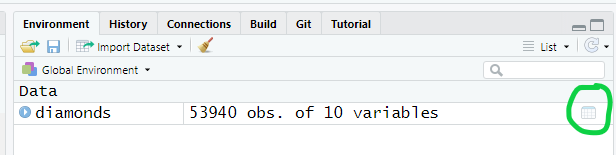
\includegraphics{../static/img/data.PNG}
\caption{\emph{screenshot of dataset in the global environment}}
\end{figure}

This area also tells us a little bit about the data set, specifically
that it has 53,940 rows and 10 variables.

When data sets are very large such as this one, it may be difficult to
see all columns or all rows. We can get an idea of the structure of the
data frame including variable names and types by using the \texttt{str}
function,

\begin{Shaded}
\begin{Highlighting}[]
\KeywordTok{str}\NormalTok{(diamonds)}
\end{Highlighting}
\end{Shaded}

\begin{verbatim}
## tibble [53,940 x 10] (S3: tbl_df/tbl/data.frame)
##  $ carat  : num [1:53940] 0.23 0.21 0.23 0.29 0.31 0.24 0.24 0.26 0.22 0.23 ...
##  $ cut    : Ord.factor w/ 5 levels "Fair"<"Good"<..: 5 4 2 4 2 3 3 3 1 3 ...
##  $ color  : Ord.factor w/ 7 levels "D"<"E"<"F"<"G"<..: 2 2 2 6 7 7 6 5 2 5 ...
##  $ clarity: Ord.factor w/ 8 levels "I1"<"SI2"<"SI1"<..: 2 3 5 4 2 6 7 3 4 5 ...
##  $ depth  : num [1:53940] 61.5 59.8 56.9 62.4 63.3 62.8 62.3 61.9 65.1 59.4 ...
##  $ table  : num [1:53940] 55 61 65 58 58 57 57 55 61 61 ...
##  $ price  : int [1:53940] 326 326 327 334 335 336 336 337 337 338 ...
##  $ x      : num [1:53940] 3.95 3.89 4.05 4.2 4.34 3.94 3.95 4.07 3.87 4 ...
##  $ y      : num [1:53940] 3.98 3.84 4.07 4.23 4.35 3.96 3.98 4.11 3.78 4.05 ...
##  $ z      : num [1:53940] 2.43 2.31 2.31 2.63 2.75 2.48 2.47 2.53 2.49 2.39 ...
\end{verbatim}

The \texttt{diamonds} data set contains numeric variables such as
\texttt{carat}, \texttt{depth}, and \texttt{price}, and ordered factor
variables including the \texttt{cut}, \texttt{color}, and
\texttt{clarity} of those diamonds.

\hypertarget{inspecting-data.frame-objects}{%
\subsection{Inspecting data.frame
objects}\label{inspecting-data.frame-objects}}

Here is a non-exhaustive list of functions to get a sense of the
content/structure of the data. Let's try them out!

\begin{itemize}
\tightlist
\item
  Size:

  \begin{itemize}
  \tightlist
  \item
    \texttt{dim(diamonds)} - returns a vector with the number of rows in
    the first element, and the number of columns as the second element
    (the dimensions of the object)
  \item
    \texttt{nrow(diamonds)} - returns the number of rows
  \item
    \texttt{ncol(diamonds)} - returns the number of columns
  \end{itemize}
\item
  Content:

  \begin{itemize}
  \tightlist
  \item
    \texttt{head(diamonds)} - shows the first 6 rows
  \item
    \texttt{tail(diamonds)} - shows the last 6 rows
  \end{itemize}
\item
  Names:

  \begin{itemize}
  \tightlist
  \item
    \texttt{names(diamonds)} - returns the column names (synonym of
    colnames() for data.frame objects)
  \item
    \texttt{rownames(diamonds)} - returns the row names
  \end{itemize}
\item
  Summary:

  \begin{itemize}
  \tightlist
  \item
    \texttt{str(diamonds)} - structure of the object and information
    about the class, length and content of each column
  \item
    \texttt{summary(diamonds)} - summary statistics for each column
  \end{itemize}
\end{itemize}

Note: most of these functions are ``generic'', they can be used on other
types of objects besides a data.frame

\hypertarget{identifying-variables}{%
\subsection{Identifying variables}\label{identifying-variables}}

Data frames can be subset by specifying indices (as shown previously),
but also by calling their column names directly:

\begin{Shaded}
\begin{Highlighting}[]
\NormalTok{diamonds[, }\StringTok{"depth"}\NormalTok{]}
\NormalTok{diamonds[, }\DecValTok{5}\NormalTok{] }
\NormalTok{diamonds}\OperatorTok{$}\NormalTok{depth}
\end{Highlighting}
\end{Shaded}

The \texttt{\$} notation has the format \texttt{data\$variable} and so
can be thought of as specifying which data set the variable is in. It is
easy to imagine a situation where two different data sets have the same
name.

This allows us to perform calculations on an individual variable. Below
is an example of finding the average price for all diamonds in the data
set.

\begin{Shaded}
\begin{Highlighting}[]
\KeywordTok{mean}\NormalTok{(diamonds}\OperatorTok{$}\NormalTok{price)}
\end{Highlighting}
\end{Shaded}

\begin{verbatim}
## [1] 3932.8
\end{verbatim}

You can also subset a variable based on the value of a secondary
variable. Here is an example of finding the average price for
\texttt{Good} quality diamonds.

\begin{Shaded}
\begin{Highlighting}[]
\KeywordTok{mean}\NormalTok{(diamonds}\OperatorTok{$}\NormalTok{price[diamonds}\OperatorTok{$}\NormalTok{cut}\OperatorTok{==}\StringTok{"Good"}\NormalTok{])}
\end{Highlighting}
\end{Shaded}

\begin{verbatim}
## [1] 3928.864
\end{verbatim}

Note that the \$ is used in both locations where we want to identify a
variable.

That's all we're covering for this week. You are ready to start the
homework!

\begin{center}\rule{0.5\linewidth}{0.5pt}\end{center}

\hypertarget{go-back-to-week-1}{%
\section{Go Back to Week 1 }\label{go-back-to-week-1}}

\begin{center}\rule{0.5\linewidth}{0.5pt}\end{center}

This material is a derivation from work that is Copyright © Software
Carpentry (\url{http://software-carpentry.org/}) which is under a
\href{https://creativecommons.org/licenses/by/4.0/}{CC BY 4.0 license}
which allows for adaptations and reuse of the work.

\end{document}
